\begin{figure}[htp]
\centering
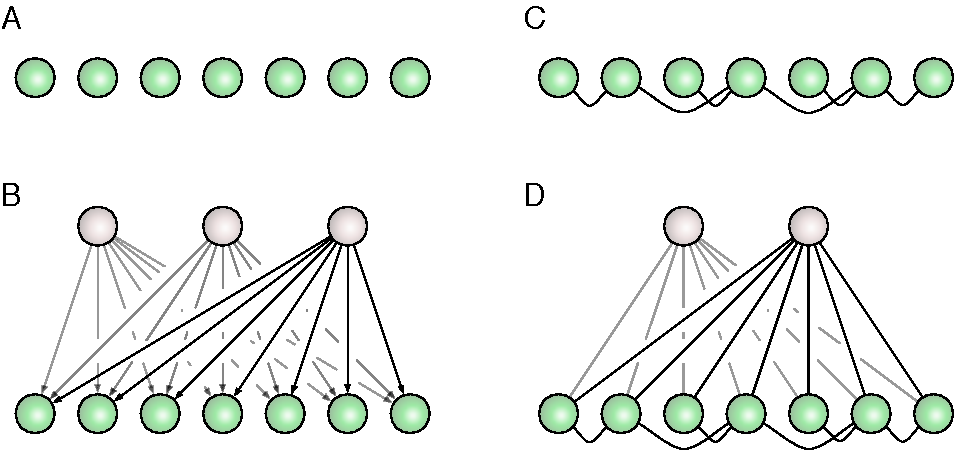
\includegraphics[width=0.5\textwidth]{figures/Figure2.pdf}
\caption{
Graphical models corresponding to the low-dimensional targets of the four regularization schemes used in the paper. It assumed that all interactions are linear, \emph{i.e.}\;the mean firing rate of any neuron can be computed by a linear combination of the firing rates of other neurons and latent units.
\textbf{A}: ``Independent.'' A population with no interactions corresponds to the diagonal covariance matrix.
\textbf{B}: ``Latent factors.'' Observed nodes are assumed to be influenced by several latent units (``factors") but are otherwise independent.
\textbf{C}: ``Sparse.'' Partial correlations between a subset of pairs of observed neurons, zero partial correlations between all other pairs.  
\textbf{D}: ``Sparse+latent.''  Partial correlations between a subset of pairs of observed neurons and a few latent factors interacting with the entire population. 
}\label{fig:02}
\end{figure}
